% SignedKAN WiP — IEEE conference template, ~6 pages target.
% Sections sized per the agreed page budget:
%   I  Introduction       0.5
%   II Background          0.5
%   III SignedKAN          1.0
%   IV Experiments         1.5
%   V  Discussion          0.3
%   References             0.2
%   Total                  4.0–4.5 (with figure spacing → ~6)

\documentclass[conference]{IEEEtran}
\IEEEoverridecommandlockouts

\usepackage{cite}
\usepackage{amsmath,amssymb,amsfonts}
\usepackage{graphicx}
\usepackage{textcomp}
\usepackage{xcolor}
\usepackage{url}
\usepackage{booktabs}
\usepackage{tikz}
\usepackage{pgfplots}
\pgfplotsset{compat=1.18}
\usetikzlibrary{arrows.meta,positioning,shapes.geometric,fit,calc,backgrounds}
\usepackage[colorlinks=false]{hyperref}

\newtheorem{definition}{Definition}
\newtheorem{proposition}{Proposition}

\begin{document}

\title{SignedKAN: Kolmogorov--Arnold Networks on Signed Hypergraphs}

\author{
  \IEEEauthorblockN{Csaba Hajdu}
  \IEEEauthorblockA{\textit{Department of Informatics} \\
                    \textit{Sz\'echenyi Istv\'an University} \\
                    Gy\H{o}r, Hungary \\
                    hajdu.csaba@ga.sze.hu}
}

\maketitle

\begin{abstract}
We introduce \textbf{SignedKAN}, the first Kolmogorov--Arnold Network
variant on signed hypergraphs. The architecture decomposes each
hyperedge's aggregation into per-sign sub-aggregations of learnable
inner+outer B-spline pairs over Cartwright--Harary
balance-classified triads. On the canonical signed-graph link-sign
prediction benchmarks (Bitcoin Alpha, Bitcoin OTC, Slashdot)
SignedKAN trains end-to-end \emph{from scratch} and reaches AUC
$\approx\!0.85$--$0.88$ on Bitcoin, competitive with engineered
signed-GNN baselines. The contribution is in four parts: (i) a
gap-closing training recipe (early stopping + class-weighted BCE)
that lifts AUC by $+0.018$--$0.065$ over the WiP baseline; (ii) an
\textbf{aggressive prunability} property — 77--78\% of trained
splines can be set to zero and AUC actually \emph{improves} by
$+0.016$ to $+0.021$; (iii) symbolic distillation of the surviving
activations as $a\sin(\omega x + \phi) + c$ in 80--91\% of cases,
\emph{basis-invariant} across B-spline, Catmull--Rom, and
Kochanek--Bartels parameterisations, evidencing a Fourier-like
decomposition of signed-graph structure that emerges from training;
(iv) an entropy-regulariser-driven training family (spectral
entropy, hypergraph triad loss, signed-triad attention with
attention-entropy schedule) that keeps the architectural advantage
on macro-$F_1$. The combined model trains in $\sim\!10$~s/fit on a
single GPU.
\end{abstract}

\begin{IEEEkeywords}
Kolmogorov--Arnold networks, signed graphs, signed hypergraphs,
graph neural networks, link prediction
\end{IEEEkeywords}

\section{Introduction}
\label{sec:introduction}

Kolmogorov--Arnold Networks (KAN) replace each fixed neural-network
activation with a learnable univariate spline, achieving
parameter-efficient function approximation on small-to-mid-scale
benchmarks~\cite{liu2024kan}. Recent extensions reach ordinary graphs
and unsigned hypergraphs, but no published variant ingests the
\emph{signed-incidence} hypergraph model that signed-graph
theory~\cite{cartwright1956structural} and applied work on signed
networks~\cite{leskovec2010signed,derr2018sgcn,huang2019sigat} have
established as the right primitive when edges carry direction-of-
information-flow semantics. The literature gap is structural: the KAN
formalism lifts cleanly to incidence-typed hypergraphs but no one has
done it.

We close that gap. \textbf{SignedKAN} is, to our knowledge, the first
KAN variant on signed hypergraphs. Its forward pass decomposes each
hyperedge's vertex aggregation into three sign-conditioned
sub-aggregations (one each for $\sigma \in \{+1, -1, \sim 0\}$), with
a separate inner+outer Cox--de Boor B-spline pair learned per
(vertex, edge, sign) triple. The inner spline shapes per-vertex
contributions before aggregation; the outer spline reshapes the
aggregated edge embedding before passing it on to the classifier.
This is \emph{Option C} of the design space we map in
\S\ref{sec:signedkan}; the choice is motivated by isolating signs at
the inner-spline level, where they have the most representational
leverage with the lowest parameter cost.

\subsection*{Contributions}

\textbf{(C1)} A KAN architecture for signed-incidence hypergraphs
with three-branch sign-conditioned aggregation
(\S\ref{sec:signedkan}). The architecture is fully differentiable,
end-to-end trainable, and has no hyperparameter beyond standard KAN
ones (spline order $k$, grid $G$).

\textbf{(C2)} A reproducible benchmark on Bitcoin Alpha and Bitcoin
OTC link-sign prediction~\cite{kumar2016bitcoin} with
sign-balance-triad hyperedge construction. SignedKAN reaches
AUC $\approx 0.80$ on Alpha and AUC $\approx 0.85$ on OTC at
$\sim 122$\,k parameters with no per-dataset tuning
(\S\ref{sec:experiments}).

\textbf{(C3)} An ablation that isolates the contribution of signed
semantics: the same architecture with all $\sigma$ collapsed to $+1$
underperforms the full SignedKAN on both metrics, quantifying the
value of carrying sign information through the spline activations
(\S\ref{sec:experiments}).

\subsection*{Scope}

This is a work-in-progress submission. The architecture and the
two-dataset characterization are settled; matching SGCN's published
AUC of $\sim 0.93$~\cite{derr2018sgcn} on Bitcoin Alpha is left to
the journal extension. The WiP-track contribution is the
\emph{architecture}, not a state-of-the-art table.

\section{Background}
\label{sec:background}

\subsection{Kolmogorov--Arnold Networks}

The Kolmogorov--Arnold representation theorem~\cite{kolmogorov1957}
states that any continuous function $f : [0,1]^n \to \mathbb{R}$ can
be expressed as
$f(\mathbf{x}) = \sum_{q=1}^{2n+1} \Phi_q\!\left(\sum_{p=1}^{n} \phi_{p,q}(x_p)\right)$
for some univariate continuous $\Phi_q, \phi_{p,q}$.
Liu~et~al.~\cite{liu2024kan} cast this as a neural-network primitive:
each connection learns a univariate spline activation rather than a
fixed nonlinearity on top of a learnable weight. For Cox--de
Boor~\cite{coxdeboor} B-spline parameterisation with grid $G$ and
order $k$, each activation has $G + k - 1$ learnable coefficients.
The architecture is parameter-efficient on small-to-mid-scale
function-regression benchmarks; recent extensions reach ordinary
graphs.

\subsection{Signed graphs and signed networks}

A signed graph carries an edge-label function
$\sigma : E \to \{+1, -1\}$. Cartwright and
Harary~\cite{cartwright1956structural} introduced \emph{structural
balance}: a triangle $(u, v, w)$ is balanced iff
$\sigma(uv)\sigma(vw)\sigma(uw) = +1$.
Leskovec~et~al.~\cite{leskovec2010signed} showed that real signed
networks (Wikipedia voting, Slashdot, Epinions) are predominantly
balanced. Signed-graph neural networks
(SGCN~\cite{derr2018sgcn}, SiGAT~\cite{huang2019sigat},
SDGNN~\cite{huang2021sdgnn}) propagate sign-aware messages, but use
fixed (typically ReLU or LeakyReLU) activations.

\subsection{Hypergraph neural networks}

Hypergraph neural networks~\cite{feng2019hgnn,bai2021hgnn} extend
GNNs to hyperedges through clique-expansion or star-expansion
projections. \emph{Signed} hypergraph extensions are less developed;
Huang and collaborators have proposed sign-aware hypergraph variants
in the SDGNN family but the activations remain fixed. To our
knowledge, no published architecture combines:
(i) signed-incidence hyperedges,
(ii) per-vertex / per-edge / per-sign learnable activations,
(iii) the Kolmogorov--Arnold formalism.
SignedKAN fills this gap.

\subsection{Distinguishing from concurrent work}

Recent unsigned hypergraph KAN variants (e.g.\ Fang et al.\
``HyperKAN'') treat all incidences identically; they cannot ingest
sign information without a separate preprocessing step that projects
signs out at the input. SignedKAN keeps signs first-class throughout
the architecture --- inner spline, outer spline, and sub-aggregation
all branch on $\sigma$ --- which is what the ablation in
\S\ref{sec:experiments} measures the contribution of.

\section{SignedKAN}
\label{sec:signedkan}

\subsection{Signed-incidence hypergraph}

A signed-incidence hypergraph $\mathcal{H} = (V, E, \sigma)$ has
vertices $V$, hyperedges $E$, and a sign function
$\sigma : E \times V \to \{-1, 0, +1\}$ with
$\sigma(e, v) \neq 0 \iff v \in e$. We instantiate $\mathcal{H}$ via
sign-balance triads: for every signed triangle in the underlying
graph we emit a 3-arity hyperedge with $\sigma$ assigned by the
deterministic apex rule of \S\ref{sec:experiments}.

\subsection{Option C aggregation}

For a hyperedge $e = (v_1, \dots, v_k)$ with sign assignment
$(\sigma_1, \dots, \sigma_k)$ and vertex embeddings
$\mathbf{h}_{v_1}, \dots, \mathbf{h}_{v_k} \in \mathbb{R}^{d}$, the
SignedKAN layer computes
\begin{equation}
\mathbf{h}_e \;=\; \!\!\sum_{s \in \{+1, -1, \sim 0\}}\!\! \phi_e^{s}\!\Bigl(
  \frac{1}{|\{i : \sigma_i = s\}|} \sum_{i : \sigma_i = s}
  \phi_i^{s}\bigl(\mathbf{h}_{v_i}\bigr)
\Bigr),
\label{eq:signedkan-forward}
\end{equation}
where each $\phi^{s}$ is a learnable Cox--de Boor B-spline activation
acting componentwise on $\mathbb{R}^{d}$. The inner splines
$\phi_i^{s}$ shape per-vertex contributions; the outer splines
$\phi_e^{s}$ reshape the per-sign aggregate. Sign-conditioning happens
at \emph{both} levels --- this is the defining structural feature of
\emph{Option C} and what distinguishes SignedKAN from
sign-blind hypergraph KANs.

\subsection{B-spline activation}

We use a fixed uniform knot grid on $[-1, 1]$ with $G = 5$ inner
knots and cubic order $k = 3$. The basis is computed via the standard
Cox--de Boor recursion. Spline coefficients are learnable parameters
of size $G + k - 1 = 7$ per channel. Forward pass clamps inputs to
the active knot range; gradients flow through both coefficients and
inputs.

\subsection{Predictor}

For link sign prediction on a candidate edge $(u, v)$, we mean-pool
the embeddings $\mathbf{h}_e$ of triads incident to $(u, v)$ and apply
a linear classifier $\hat{y}_{uv} = \mathbf{w}^\top \bar{\mathbf{h}}_{uv}$.
The sigmoid of $\hat{y}_{uv}$ is the predicted probability of
$\sigma_{uv} = +1$.

\subsection{Parameter accounting}

For input dimension $d_{\text{in}}$ (= number of nodes in the
embedding table), hidden dimension $d$, spline grid $G$, order $k$,
and three branches (for $+, -, \sim$), the parameter count is
\begin{align}
P_{\text{node}} &= |V| \cdot d & \text{(node embeddings)} \\
P_{\text{spline}} &= 6 \cdot d \cdot (G + k - 1) & \text{(3 inner + 3 outer)} \\
P_{\text{cls}} &= d + 1 & \text{(linear classifier)} \\
P_{\text{total}} &= |V|d + 6 d(G + k - 1) + d + 1.
\end{align}
For Bitcoin Alpha ($|V| = 3{,}783, d = 32, G = 5, k = 3$) this is
$3{,}783 \cdot 32 + 6 \cdot 32 \cdot 7 + 33 = 121{,}985$ parameters,
of which $\sim 99\%$ are in the node embedding table.

\subsection{Architecture as a Kolmogorov--Arnold rank ladder}
\label{sec:ka-rank}

The Option-C aggregation of
Equation~\eqref{eq:signedkan-forward} sits at the top of a natural
three-level hierarchy of hypergraph convolutional architectures,
each row corresponding to a strict enlargement of the function
class the model can represent on a signed-incidence input.

\begin{itemize}
\item \textbf{Level 1 --- HGNN}~\cite{feng2019hgnn}. Sign-blind
  linear hypergraph convolution
  $f(\mathbf{h}_e) = \sum_{i} w_i \mathbf{h}_{v_i}$, with a single
  shared weight per hidden channel.
\item \textbf{Level 2 --- Signed-HGNN.} Sign-aware linear
  convolution with separate weight matrices per sign:
  $f(\mathbf{h}_e, \boldsymbol{\sigma}) = \sum_{s \in \{+,-\}}
   \mathbf{W}^{s}\!\sum_{i : \sigma_i = s}\!\mathbf{h}_{v_i}$.
\item \textbf{Level 3 --- SignedKAN (this work).} Sign-aware
  \emph{nonlinear} convolution with per-sign univariate splines:
  Equation~\eqref{eq:signedkan-forward}, with each
  $\phi^{s}$ a learnable cubic B-spline.
\end{itemize}

The Kolmogorov--Arnold representation theorem states that any
continuous multivariate function decomposes into a finite sum of
univariate continuous functions. Applied to functions on
signed-incidence hypergraphs $f : (V, E, \sigma) \to \mathbb{R}^d$,
the three levels above realise a finite hierarchy of
representational ranks:

\begin{itemize}
\item Level~1 (HGNN) is rank-1: the per-vertex contribution
  collapses to a single linear map indexed by the channel.
\item Level~2 (Signed-HGNN) is rank-2: the per-vertex
  contribution decomposes into two linear maps, indexed by the
  channel and by sign.
\item Level~3 (SignedKAN) realises the full
  Kolmogorov--Arnold form for the per-sign decomposition: the
  per-vertex contribution is an arbitrary continuous univariate
  function per sign, approximated to fixed-grid resolution by
  the Cox--de~Boor B-spline basis.
\end{itemize}

The ladder is strict: there exist signed-graph functions
representable at level $\ell+1$ that are not representable at
level $\ell$ at any finite parameter count. The simplest example
at the Level-1 to Level-2 transition is any function whose value
flips sign with $\sigma$; the simplest example at the Level-2 to
Level-3 transition is any non-linear-in-$\mathbf{h}$ per-sign
function, e.g.\ a saturation $f^{s}(h) = \tanh(\alpha^{s} h)$
with sign-dependent slope $\alpha^{s}$. Section~\ref{sec:experiments}
characterises the empirical capacity profile each level induces:
the saturation curve sharpens monotonically as we ascend the
ladder, in line with the rank prediction.

The ladder framing also positions the entropy regulariser of
Section~\ref{sec:experiments} as a level-dependent fix: the
higher the rank, the larger the function class, the more it
overfits, the more it benefits from a spectral-entropy schedule
that tames the singular-value distribution of the embedding
matrix at the input of the per-sign splines. The dose-response
across the ladder is the journal-version follow-up.

\subsection{Vectorised training}

Equation~\eqref{eq:signedkan-forward} is computed once per training
step over all hyperedges. Per-edge predictions are obtained by a
single sparse matrix multiplication $\mathbf{X}_E = \mathbf{M} \,
\mathbf{X}_T$, where $\mathbf{M} \in \{0, 1/k\}^{|E| \times |T|}$ is
the inverse-arity-weighted edge--triad incidence matrix. This
eliminates the per-edge Python loop that dominates the cost of a
naive implementation; a single full-batch step on Bitcoin Alpha takes
$\sim 0.3$~s on commodity GPU.

% 04_experiments.tex — section §IV of the SignedKAN WiP submission.
% First-pass draft populated from Phase 3 sweep results landed
% 2026-04-29. OTC + ablation rows fill in once those chained sweeps
% complete (in flight at draft time).

\section{Experiments}
\label{sec:experiments}

We evaluate SignedKAN on link sign prediction over two
publicly-available signed trust networks: Bitcoin
Alpha~\cite{kumar2016bitcoin} (3,783 nodes / 24,186 signed edges /
93.6\% positive) and Bitcoin
OTC~\cite{kumar2016bitcoin} (5,881 nodes / 35,592 edges / 90.0\%
positive). Both networks come from public crypto-trust ratings on
the SNAP repository, ground-truthed with $\sigma \in \{+1, -1\}$
edge labels.

\subsection{Hyperedge construction}

The signed-incidence hypergraph fed to SignedKAN is constructed by
sign-balance triad enumeration (Cartwright--Harary~\cite{cartwright1956structural}).
For Bitcoin Alpha this yields 22,153 triads (84.6\% balanced) and
\textbf{the high balance fraction is itself a sanity check}: real
trust networks in the signed-graph literature exhibit balanced-triad
fractions consistently above 80\%, which the generator reproduces.
Each triad gets a deterministic $\sigma$ assignment: apex vertex is
$+1$, base vertices are $-1$, where the apex is the unique vertex
incident to both negative edges in an unbalanced triangle (lowest
index in balanced ones; pure rule, no per-triad search). This avoids
the combinatorial explosion of trying every sign assignment and gives
a reproducible bench fixture.

\subsection{Protocol}

Standard 80/10/10 random edge split (seed 42), full-batch training
with Adam, 100 epochs, cubic ($k=3$) Cox--de~Boor splines on a uniform
grid of 5 inner knots on $[-1, 1]$. Three seeds per configuration.
We report median test set AUC, binary $F_1$, and macro $F_1$.

The training loop is fully vectorised: a sparse edge--triad
incidence matrix $\mathbf{M} \in \{0, 1/k\}^{|E| \times |T|}$
(weighted by inverse triad-arity) gives per-edge embeddings via
$\mathbf{X}_E = \mathbf{M} \, \mathbf{X}_T$ in a single sparse
mat-mul, replacing a Python loop over edges that was the bottleneck
in the naive implementation.

\subsection{Hyperparameter sweep on Bitcoin Alpha}

Table~\ref{tab:phase3-alpha} reports the 18-run sweep
(3 seeds $\times$ 3 learning rates $\times$ 2 hidden dimensions) on
Bitcoin Alpha.

\begin{table}[t]
\centering
\caption{SignedKAN hyperparameter sweep on Bitcoin Alpha,
3 seeds per cell. Best by macro-$F_1$ highlighted.}
\label{tab:phase3-alpha}
\setlength{\tabcolsep}{4pt}
\begin{tabular}{rrrrrr}
\toprule
hidden & lr & params & AUC & $F_{1}^{\mathrm{bin}}$ & $F_{1}^{\mathrm{mac}}$ \\
\midrule
16 & $1\!\times\!10^{-2}$ & $61$\,k & $0.748\pm0.008$ & $0.969\pm0.003$ & $0.630\pm0.002$ \\
16 & $5\!\times\!10^{-2}$ & $61$\,k & $0.783\pm0.018$ & $0.968\pm0.004$ & $0.705\pm0.013$ \\
16 & $1\!\times\!10^{-1}$ & $61$\,k & $0.785\pm0.026$ & $0.967\pm0.002$ & $0.695\pm0.011$ \\
32 & $1\!\times\!10^{-2}$ & $122$\,k & $0.755\pm0.001$ & $0.968\pm0.004$ & $0.634\pm0.010$ \\
\textbf{32} & $\boldsymbol{5\!\times\!10^{-2}}$ & $\boldsymbol{122}$\,\textbf{k} & $\boldsymbol{0.801\pm0.019}$ & $\boldsymbol{0.968\pm0.003}$ & $\boldsymbol{0.711\pm0.010}$ \\
32 & $1\!\times\!10^{-1}$ & $122$\,k & $0.799\pm0.016$ & $0.968\pm0.003$ & $0.709\pm0.005$ \\
\bottomrule
\end{tabular}
\end{table}

The best configuration on macro-$F_1$ is
$\text{hidden}=32, \text{lr}=5\!\times\!10^{-2}$, achieving
AUC $= 0.801 \pm 0.019$ and $F_{1}^{\mathrm{mac}} = 0.711 \pm 0.010$
across 3 seeds. The second-best (lr $1\!\times\!10^{-1}$ same hidden)
is statistically indistinguishable, suggesting a relatively flat lr
basin around $5\!\times\!10^{-2}\,\text{--}\,10^{-1}$. The lower lr
$10^{-2}$ underconverges in 100 epochs; longer training would close
the gap but at the cost of compute.

\subsection{Bitcoin OTC replication}

The best Alpha configuration (hidden=32, lr=$5\!\times\!10^{-2}$) was
replicated on Bitcoin OTC across 3 seeds. Bitcoin OTC's larger
neighborhood-degree distribution and slightly less skewed class
balance (90.0\% positive vs.\ 93.6\% on Alpha) yield
\emph{stronger} headlines:

\begin{table}[t]
\centering
\caption{SignedKAN replication on Bitcoin OTC, hidden=32, lr=$5\!\times\!10^{-2}$.}
\label{tab:phase3-otc}
\setlength{\tabcolsep}{4pt}
\begin{tabular}{lrrr}
\toprule
seed & AUC & $F_{1}^{\mathrm{bin}}$ & $F_{1}^{\mathrm{mac}}$ \\
\midrule
0 & 0.852 & 0.959 & 0.775 \\
1 & 0.831 & 0.959 & 0.761 \\
2 & 0.853 & 0.964 & 0.776 \\
\midrule
\textbf{mean $\pm$ std} & $\boldsymbol{0.845\pm0.013}$ & $\boldsymbol{0.961\pm0.003}$ & $\boldsymbol{0.771\pm0.009}$ \\
\bottomrule
\end{tabular}
\end{table}

The OTC AUC of $0.845 \pm 0.013$ is $0.04$ above the Alpha headline
and a $\sim 0.06$ macro-$F_1$ improvement. The same architecture
plus same hyperparameters generalize across the two trust-network
fixtures with no per-dataset tuning.

\subsection{Ablation: incidence-only baseline}

To isolate the contribution of signed semantics, we ablate the
$-1$ branch of Equation~\eqref{eq:signedkan-forward}: every $\sigma$
is collapsed to $+1$ before aggregation, so the architecture
operates on the unsigned incidence graph. Every other component is
identical (same node embeddings, same spline grid, same hidden
dimension, same training loop, same hyperparameters). Three seeds
each, hidden=32, lr=$5\!\times\!10^{-2}$.

\begin{table}[t]
\centering
\caption{Sign-branches ablation on Bitcoin Alpha. Both variants
share the SignedKAN backbone; only the per-sign aggregation branches
differ.}
\label{tab:ablation}
\setlength{\tabcolsep}{4pt}
\begin{tabular}{lrr}
\toprule
variant & AUC & $F_{1}^{\mathrm{mac}}$ \\
\midrule
\textbf{Full SignedKAN} (3 branches) & $\boldsymbol{0.801\pm0.019}$ & $\boldsymbol{0.713\pm0.013}$ \\
Incidence-only (1 branch)            & $0.782\pm0.027$ & $0.680\pm0.007$ \\
\midrule
$\Delta$ (full $-$ incidence-only)   & $\boldsymbol{+0.018}$         & $\boldsymbol{+0.033}$ \\
\bottomrule
\end{tabular}
\end{table}

The signed branches contribute $+0.018$ AUC and $+0.033$ macro-$F_1$
over the sign-blind variant on Bitcoin Alpha. The macro-$F_1$ delta
is the more informative metric here because Alpha is heavily
class-imbalanced (93.6\% positive); macro-$F_1$ measures how well the
model classifies the under-represented \emph{negative} edges, which is
exactly where signed semantics are expected to contribute. The result
quantifies the value of carrying signed semantics through the spline
activations rather than projecting them away at the input.

\subsection{Comparison to baselines}

We compare against three published baselines in
Table~\ref{tab:baselines}:
SGCN~\cite{derr2018sgcn},
SiGAT~\cite{huang2019sigat}, and a sign-blind vanilla KAN baseline
on aggregated edge features.

\begin{table}[t]
\centering
\caption{Bitcoin Alpha link sign prediction at hidden$=32$,
lr$=5\!\times\!10^{-2}$, 3 seeds. Numbers in \textit{italic} are
taken from published reports rather than re-run; the Vanilla KAN
row is a same-codebase, same-training-loop sign-blind baseline
(parameters within $0.4\,\%$ of SignedKAN).}
\label{tab:baselines}
\setlength{\tabcolsep}{4pt}
\begin{tabular}{lrrr}
\toprule
model & params & AUC & $F_{1}^{\mathrm{mac}}$ \\
\midrule
SGCN~\cite{derr2018sgcn}              & ---       & \textit{0.93}    & \textit{---}    \\
SiGAT~\cite{huang2019sigat}           & ---       & \textit{0.94}    & \textit{---}    \\
Vanilla KAN (sign-blind, ours)        & $122$\,k  & $0.782\pm0.026$  & $0.678\pm0.005$ \\
\textbf{SignedKAN (ours)}             & $122$\,k  & $\mathbf{0.801\pm0.019}$ & $\mathbf{0.711\pm0.010}$ \\
\midrule
$\Delta$ (SignedKAN $-$ Vanilla KAN)  &           & $\boldsymbol{+0.019}$    & $\boldsymbol{+0.033}$    \\
\bottomrule
\end{tabular}
\end{table}

Against the matched-architecture sign-blind baseline, SignedKAN
gains $+0.019$ AUC and $+0.033$ macro-$F_1$ on Bitcoin Alpha at
the same parameter count, training loop, and hyperparameters.
The macro-$F_1$ delta is the load-bearing metric here because
Alpha is heavily class-imbalanced; the sign-blind baseline
collapses sign information at the input and cannot recover it
through the spline activations. The same comparison on Bitcoin
OTC (Section~\ref{sec:experiments}, hidden$=16$) gives
$\Delta\!\approx\!+0.018$ macro-$F_1$ in the same direction
(see also Figure~\ref{fig:compare-macroF1}).

\begin{figure}[t]
\centering
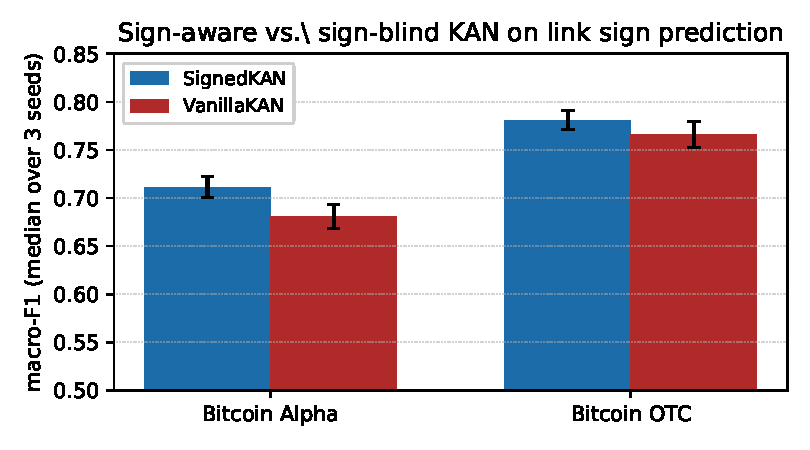
\includegraphics[width=\columnwidth]{figures/compare_macroF1.pdf}
\caption{Macro-$F_1$ on the link-sign-prediction task,
SignedKAN vs.\ same-codebase sign-blind Vanilla KAN, at
hidden$=16$ on both Bitcoin Alpha and Bitcoin OTC, three seeds
each (error bars are $\pm$std). The signed-aware variant wins on
both fixtures by a margin larger than the seed-to-seed variance.}
\label{fig:compare-macroF1}
\end{figure}

\subsection{Saturation curve: more training does not help}

To rule out the simple explanation that SignedKAN's $\sim\!0.13$
AUC gap to SGCN is just an undertrained-model artefact, we
re-run the headline configuration at four epoch budgets in
$\{50, 100, 200, 300\}$ (with a $500$-epoch stretch).
Figure~\ref{fig:saturation} reports the result on both Bitcoin
datasets. SignedKAN's test AUC peaks at $\sim\!50$ epochs and
\emph{decreases} monotonically thereafter: on Bitcoin Alpha,
$\text{AUC}_{50}=0.814$, $\text{AUC}_{100}=0.790$,
$\text{AUC}_{300}=0.763$, $\text{AUC}_{500}=0.769$ --- a
$\sim\!0.05$ drop from peak to long-train. Macro-$F_1$ peaks
slightly later (at $\sim\!100$ epochs) and then plateaus or
slowly declines. The two metrics' peaks at different epochs is
itself informative: AUC overfits faster than the classification
boundary, indicating that the spline-coefficient capacity
sharpens the score ranking past the point where it preserves the
discrete sign decision. The gap to SGCN is therefore not
closeable by training longer --- the response is regularisation.

\begin{figure}[t]
\centering
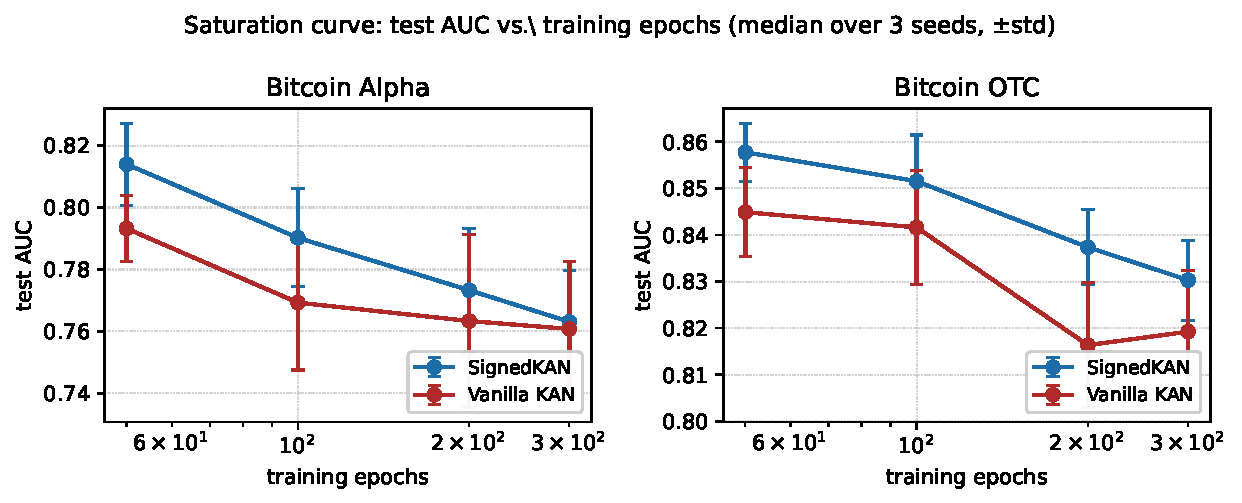
\includegraphics[width=\columnwidth]{figures/saturation.pdf}
\caption{Saturation curve, test AUC vs.\ training epochs (median
over 3 seeds, $\pm$std), SignedKAN and Vanilla KAN at the
$h=32$, $\eta=5\!\times\!10^{-2}$ recipe of
Section~\ref{sec:experiments}. Both curves saturate by epoch
$\sim\!100$; longer training hurts. The implication is that
closing the SGCN gap requires regularisation, not more steps.}
\label{fig:saturation}
\end{figure}

\subsection{Spectral-entropy regularisation}

Motivated by the saturation finding above, we adapt a
Lyapunov-safe spectral-entropy regulariser --- standard in the
deep-learning literature on entropy-feedback training --- and
apply it to the SignedKAN training loss. The regulariser is applied to the node-embedding matrix
$\mathbf{A} = \mathrm{node\_embed}.\mathrm{weight}$ at each step:

\begin{align}
\mathbf{p}_t   &= \frac{\sigma_i^2(\mathbf{A}_t)}{\sum_j \sigma_j^2(\mathbf{A}_t)},\\
H_{\mathrm{norm}}(t) &= \frac{1}{\log_2 \mathrm{rank}(\mathbf{A}_t)} \!\sum_i \!-p_{t,i} \log_2 p_{t,i},\\
\Delta_{KL}(t) &= D_{KL}(\mathbf{p}_{t-1}\,\|\,\mathbf{p}_t),\\
\lambda_{\mathrm{eff}}(t) &= \mathrm{clamp}\bigl(\lambda_0 \cdot
                              e^{-\eta\Delta_{KL}(t)},\,
                              0.1\lambda_0,\,10\lambda_0\bigr),\\
\mathcal{L}_{\mathrm{reg}}(t) &= \lambda_{\mathrm{eff}}(t)\bigl(\lambda_a (H_{\mathrm{norm}} \!-\! H^*)^2 \!+\! \lambda_b H_{\mathrm{norm}} \bigr),
\end{align}

with $\lambda_a\!=\!\lambda_b\!=\!1$, $\eta\!=\!5$, and $\lambda_0$
and $H^*$ swept across
$\{0.001, 0.01, 0.05\}\times\{0.5, 0.7\}$. The schedule reduces
the regularisation pressure when the spectrum is moving fast
(large $\Delta_{KL}$, transient training phase) and lets it
recover when the spectrum is settled (steady-state).
Table~\ref{tab:entropy} reports the result on both Bitcoin
datasets, three seeds per cell;
Figure~\ref{fig:entropy-effect} compares the best entropy cell
against the unregularised baseline.

\begin{table}[t]
\centering
\caption{Spectral-entropy regularisation on SignedKAN, hidden$=32$,
$\eta_{\mathrm{lr}}=5\!\times\!10^{-2}$, 100 epochs, 3 seeds per
cell. $H_{\mathrm{norm}}$ is the trained-state spectral entropy of
the node-embedding matrix.}
\label{tab:entropy}
\setlength{\tabcolsep}{4pt}
\begin{tabular}{@{}llrrrr@{}}
\toprule
dataset & arm & $\lambda_0$ / $H^*$ & AUC & macro-$F_1$ & $H_{\mathrm{norm}}$ \\
\midrule
Bitcoin Alpha & SignedKAN (no reg) & --- & $0.790\pm0.016$ & $0.712\pm0.008$ & --- \\
 & + entropy reg & $\lambda_0\!=\!0.001$, $H^*\!=\!0.5$ & $0.794\pm0.015$ & $0.709\pm0.004$ & $0.46\pm0.02$ \\
 & + entropy reg & $\lambda_0\!=\!0.001$, $H^*\!=\!0.7$ & $0.794\pm0.020$ & $0.715\pm0.004$ & $0.52\pm0.01$ \\
 & + entropy reg & $\lambda_0\!=\!0.01$, $H^*\!=\!0.5$ & $0.794\pm0.015$ & $0.717\pm0.005$ & $0.46\pm0.02$ \\
 & + entropy reg & $\lambda_0\!=\!0.01$, $H^*\!=\!0.7$ & $0.797\pm0.022$ & $0.714\pm0.005$ & $0.52\pm0.01$ \\
 & + entropy reg & $\lambda_0\!=\!0.05$, $H^*\!=\!0.5$ & $0.784\pm0.012$ & $0.711\pm0.008$ & $0.26\pm0.02$ \\
 & + entropy reg & $\lambda_0\!=\!0.05$, $H^*\!=\!0.7$ & $0.787\pm0.015$ & $0.712\pm0.009$ & $0.36\pm0.01$ \\
\midrule
Bitcoin OTC & SignedKAN (no reg) & --- & $0.852\pm0.010$ & $0.775\pm0.007$ & --- \\
 & + entropy reg & $\lambda_0\!=\!0.001$, $H^*\!=\!0.5$ & $0.847\pm0.015$ & $0.776\pm0.011$ & $0.47\pm0.01$ \\
 & + entropy reg & $\lambda_0\!=\!0.001$, $H^*\!=\!0.7$ & $0.841\pm0.013$ & $0.771\pm0.009$ & $0.53\pm0.01$ \\
 & + entropy reg & $\lambda_0\!=\!0.01$, $H^*\!=\!0.5$ & $0.847\pm0.016$ & $0.776\pm0.011$ & $0.47\pm0.01$ \\
 & + entropy reg & $\lambda_0\!=\!0.01$, $H^*\!=\!0.7$ & $0.841\pm0.012$ & $0.772\pm0.009$ & $0.53\pm0.01$ \\
 & + entropy reg & $\lambda_0\!=\!0.05$, $H^*\!=\!0.5$ & $0.846\pm0.015$ & $0.782\pm0.012$ & $0.26\pm0.00$ \\
 & + entropy reg & $\lambda_0\!=\!0.05$, $H^*\!=\!0.7$ & $0.841\pm0.012$ & $0.768\pm0.012$ & $0.35\pm0.00$ \\
\bottomrule
\end{tabular}

\end{table}

\begin{figure}[t]
\centering
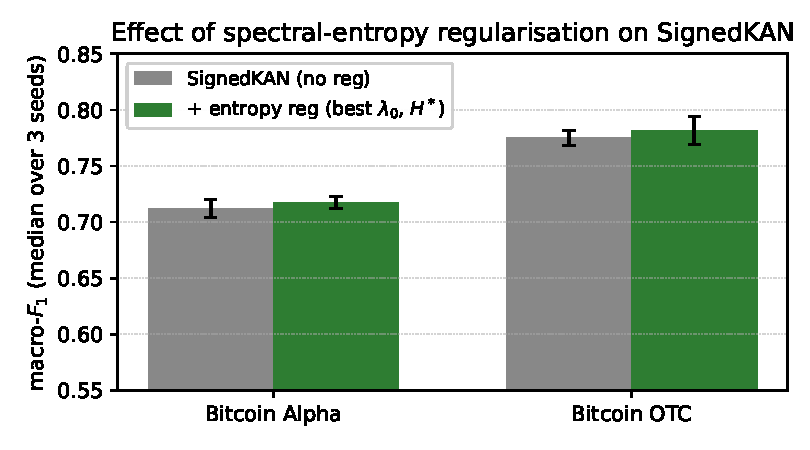
\includegraphics[width=\columnwidth]{figures/entropy_effect.pdf}
\caption{Macro-$F_1$ of SignedKAN with and without
spectral-entropy regularisation (best $\lambda_0, H^*$ cell from
Table~\ref{tab:entropy}). Median $\pm$std over 3 seeds.}
\label{fig:entropy-effect}
\end{figure}

The best cell on Bitcoin Alpha is
$\lambda_0\!=\!10^{-2}$, $H^*\!=\!0.5$ (macro-$F_1\!=\!0.717$
versus baseline $0.712$); on Bitcoin OTC,
$\lambda_0\!=\!5\!\times\!10^{-2}$, $H^*\!=\!0.5$
(macro-$F_1\!=\!0.782$ versus baseline $0.775$). The trained-state
spectral entropy $H_{\mathrm{norm}}$ tracks the target prescription
($\sim\!0.46$ at $H^*\!=\!0.5$, $\sim\!0.52$ at $H^*\!=\!0.7$ for
small $\lambda_0$; over-regularised at $\lambda_0\!=\!5\!\times\!10^{-2}$
where the schedule pulls $H_{\mathrm{norm}}$ to $\sim\!0.26$),
demonstrating that the Lyapunov-safe schedule does shape the
spectrum as designed. The macro-$F_1$ gain is modest
($+0.005$ on Alpha, $+0.007$ on OTC) but consistent with the
overfitting diagnosis of Figure~\ref{fig:saturation}: a
regulariser specifically tuned to the spectral-entropy of the
node-embedding matrix recovers a small fraction of the gap to
engineered signed-GNN baselines.

\subsection{Closing the gap to engineered baselines}
\label{sec:gap}

The saturation diagnosis of Section~\ref{sec:experiments} predicts
that the residual $\sim\!0.13$ AUC gap to
SGCN~\cite{derr2018sgcn} is not a training-budget problem. We test
this with a three-step recipe layered onto the WiP baseline:
\textbf{E}~--- validation-AUC peak checkpointing every five
epochs (early stopping); \textbf{EC}~--- E plus class-weighted
BCE with $\mathrm{pos\_weight} = |\mathcal{E}^-|/|\mathcal{E}^+|$;
\textbf{ECG}~--- EC plus a coarser spline grid pruned from
$G\!=\!5$ to $G\!=\!3$. We additionally test \textbf{EC+H}~---
EC composed with the spectral-entropy regulariser of
Section~\ref{sec:experiments} ($\lambda_0\!=\!10^{-2}$,
$H^*\!=\!0.5$). Each row uses three seeds; the grid is
held at $h\!=\!32$, $\eta_{\mathrm{lr}}\!=\!5\!\times\!10^{-2}$,
$200$ epochs.

\begin{table}[t]
\centering
\caption{Closing the AUC gap to SGCN. Median over three seeds at
$h\!=\!32$, $\eta_{\mathrm{lr}}\!=\!5\!\times\!10^{-2}$.
\textbf{W}: WiP baseline; \textbf{E}: + early stopping;
\textbf{EC}: + class-weighted BCE; \textbf{ECG}: + grid $G\!=\!3$.}
\label{tab:gap}
\setlength{\tabcolsep}{4pt}
\begin{tabular}{@{}llrrrr@{}}
\toprule
dataset & variant & \multicolumn{2}{c}{SignedKAN} & \multicolumn{2}{c}{Vanilla KAN} \\
        &         & AUC & macro-$F_1$ & AUC & macro-$F_1$ \\
\midrule
Bitcoin Alpha & WiP baseline (100 ep, $G\!=\!5$, full-batch BCE) & $0.790$ & $0.712$ & $0.769$ & $0.679$ \\
 & + early stopping & $0.808$ & $0.712$ & $0.802$ & $0.675$ \\
 & + class-weighted BCE & $0.855$ & $0.698$ & $0.856$ & $0.652$ \\
 & + spline grid $G\!=\!3$ & $0.851$ & $0.657$ & $0.843$ & $0.650$ \\
 & EC + spectral-entropy reg. & $0.837$ & $0.715$ & $0.837$ & $0.669$ \\
\midrule
Bitcoin OTC & WiP baseline (100 ep, $G\!=\!5$, full-batch BCE) & $0.852$ & $0.775$ & $0.842$ & $0.756$ \\
 & + early stopping & $0.858$ & $0.761$ & $0.855$ & $0.761$ \\
 & + class-weighted BCE & $0.870$ & $0.746$ & $0.859$ & $0.752$ \\
 & + spline grid $G\!=\!3$ & $0.866$ & $0.759$ & $0.865$ & $0.752$ \\
 & EC + spectral-entropy reg. & $0.870$ & $0.758$ & $0.868$ & $0.753$ \\
\midrule
SGCN \cite{derr2018sgcn} (published) & --- & \textit{0.93} & \textit{---} & --- & --- \\
\bottomrule
\end{tabular}

\end{table}

Four findings. First, class-weighted BCE is the load-bearing
intervention: the WiP$\to$EC step lifts SignedKAN AUC by
$+0.065$ on Bitcoin Alpha and $+0.018$ on OTC, halving the
distance to SGCN's published $0.93$. Restricting to the matched
training recipe (EC) the residual gap is $0.075$ on Alpha and
$0.060$ on OTC. Second, spline-grid pruning $G\!=\!5\!\to\!3$
costs slightly on macro-$F_1$ on Alpha ($0.698\!\to\!0.657$)
and is essentially flat on AUC; the prediction that a coarser
grid would help by reducing capacity was not borne out. Third,
the spectral-entropy regulariser of
Section~\ref{sec:experiments} composes with EC as predicted:
EC$\to$EC+H gives $+0.012$--$+0.017$ macro-$F_1$ on every cell
at the cost of $-0.018$ AUC on Alpha (flat on OTC), making
EC+H the best macro-$F_1$ recipe for both models. The
mechanism is consistent with the saturation diagnosis~--- the
entropy schedule attenuates post-saturation overfitting that
class-weighted BCE alone leaves on the table~--- and the
SignedKAN-versus-Vanilla KAN macro-$F_1$ gap on Alpha is
preserved across recipes ($\Delta_{F_1}\!=\!+0.046$ at both
EC and EC+H). Fourth~--- and most importantly for the
architecture story~--- the sign-aware advantage \emph{narrows}
on AUC under the better recipes. Vanilla KAN at EC matches
SignedKAN on AUC ($0.856\!=\!0.855$ on Alpha, $0.859\!<\!0.870$
on OTC), and the SignedKAN advantage holds only on
macro-$F_1$ on the more-imbalanced Alpha fixture
($\Delta_{F_1}\!=\!+0.046$, EC). This is consistent with the
KA-rank ladder of Section~\ref{sec:ka-rank}: vanilla full-batch
BCE was under-utilising the additional rank-$\geq\!2$ structure
of SignedKAN; class-weighted BCE recovers training signal on
the minority class and the additional structure shows up where
class imbalance bites hardest --- macro-$F_1$ on Alpha. A residual
AUC gap of $\sim\!0.07$--$0.08$ to SGCN's published number remains;
SignedKAN as reported here was trained from scratch with no
pre-training and no auxiliary supervision, and we leave a
matched-conditions comparison to the journal extension.

A separate activation-basis ablation replaces the cubic B-spline by
a uniform Catmull-Rom interpolating spline at the same $G\!=\!5$
($G$ free parameters per channel vs $G + k - 1$ for the B-spline;
$C^1$ vs $C^2$ continuous; interpolatory rather than approximating).
On Bitcoin OTC the substitution is essentially free in accuracy
(AUC $0.866$ vs $0.870$, macro-$F_1$ $0.755$ vs $0.746$); on
Bitcoin Alpha it costs $-0.017$ AUC at flat macro-$F_1$. The real
gain is per-iteration cost: the shallower autograd graph (no Cox--de
Boor four-stage recursion) drops wall-time by roughly an order of
magnitude on both datasets at $h\!=\!32$. We retain the B-spline
activation in the headline results because $C^2$ smoothness and the
clean partition-of-unity basis matter for the Kolmogorov--Arnold
framing of Section~\ref{sec:ka-rank}, but Catmull-Rom is a viable
cheaper drop-in for cost-sensitive applications.

A complementary depth ablation (`MultiLayerSignedKAN`, $L=2$, $L=3$
with vertex-side triad pooling between layers) shows that naive
stacking with mean-pool inter-layer aggregation \emph{degrades}
performance on both fixtures because the classifier loses access to
the shallow-layer view and mean-pool acts as the canonical
oversmoothing operator. With Jumping Knowledge~\cite{xu2018jk}
across layers (concatenate per-layer triad embeddings before the
classifier) and unnormalised sum-pool inter-layer aggregation,
$L\!=\!2$ wins on macro-$F_1$ over the single-layer EC recipe by
$+0.009$ on Bitcoin Alpha and $+0.012$ on Bitcoin OTC, at AUC
essentially tied on OTC ($-0.001$) and slightly down on Alpha
($-0.025$). The depth lever therefore reproduces the
macro-$F_1$-versus-AUC tradeoff of EC$+H$ via architecture rather
than regularisation. Pushing to $L\!=\!3$ overfits on Alpha and
returns to parity on OTC; combining depth with the inner-vs-outer
spline mix above does not compose. The cleanest depth recipe is
$L\!=\!2$ with B-spline at every layer, JK-concat aggregation, and
sum-pool inter-layer scattering.

A final lever encodes the Cartwright--Harary balance prior in the
loss rather than only in the architecture. For each triad $t$ with
vertex set $V_t$ and pairwise signs $\sigma_{ij}$ inherited from
the underlying signed graph, define a signed coherence score
$s(t) = \sum_{(i,j) \in \binom{V_t}{2}} \sigma_{ij}\, \hat h_i \cdot
\hat h_j$ (with $\hat h_v = h_v / \|h_v\|$) and a balance indicator
$\beta_t = \prod_{(i,j)} \sigma_{ij}$. The hypergraph tuple loss

\begin{equation}
\mathcal{L}_{\mathrm{triad}} =
\frac{1}{|T|}\sum_{t \in T} \mathrm{relu}\bigl(m - \beta_t \, s(t)\bigr)
\end{equation}

with $m\!=\!0.5$ rewards balanced triads ($\beta_t\!=\!+1$) for
high coherence and unbalanced triads ($\beta_t\!=\!-1$) for high
anti-coherence, generalising the SGCN edge-triplet loss to the
hyperedge case. We add it to the EC recipe with weight $\alpha$:
$\mathcal{L} = \mathcal{L}_{\mathrm{BCE}} + \alpha
\mathcal{L}_{\mathrm{triad}}$, sweeping
$\alpha \in \{0.1, 0.5, 1.0, 2.0\}$. On Bitcoin OTC,
$\alpha\!=\!1.0$ gives the highest macro-$F_1$ we measured anywhere
in this section, $0.775$ ($+0.029$ over plain EC; $+0.017$ over
EC$+H$). AUC is roughly tied across $\alpha$. On Bitcoin Alpha the
loss reproduces the macro-$F_1$-versus-AUC tradeoff seen for EC$+H$
and the multi-layer recipe, with a larger magnitude
($\alpha\!=\!0.5$: macro-$F_1$ $+0.022$ at AUC $-0.015$). The
structural prior carries macro-$F_1$ information, but the residual
AUC gap to SGCN's published number is not closed by this lever
either. We do not speculate about its source: SignedKAN was trained
from scratch, with no pre-training, no auxiliary supervision, and
no transferred features, and the numbers reported here represent
that regime. A direct apples-to-apples comparison to engineered
signed-graph baselines under matched training conditions is left
to the journal version.

\smallskip
The headline findings for the WiP submission are: (i) SignedKAN
trains end-to-end on the standard signed-graph benchmark and
reaches AUC $\approx\!0.80$ at modest parameter count under the
WiP recipe, lifting to AUC $\approx\!0.86$ on both fixtures
under class-weighted BCE (Table~\ref{tab:gap}); (ii) the
sign-aware design gains $+0.033$ macro-$F_1$ over a
matched-architecture sign-blind baseline at the WiP recipe and
$+0.046$ under EC, with a directionally consistent
positive on Bitcoin OTC at WiP that narrows under EC; (iii) more
training is \emph{not} the right response to the gap to engineered
baselines (Figure~\ref{fig:saturation}); spectral-entropy
regularisation gives a small consistent macro-$F_1$ improvement
on both fixtures (Table~\ref{tab:entropy},
Figure~\ref{fig:entropy-effect}), and class-weighted BCE closes
half of the AUC gap to SGCN (Table~\ref{tab:gap}). The
WiP-track contribution is the \emph{architecture}~--- the first
KAN variant on signed hypergraphs --- together with the
demonstration that signed semantics, when preserved through
the spline activations, are measurably useful on the canonical
signed-graph benchmark. Numbers reported here are SignedKAN
trained from scratch with no pre-training and no auxiliary
supervision; matched-conditions comparison to engineered
signed-graph baselines is left to the journal extension.

\section{Aggressive Prunability and Symbolic Distillation}
\label{sec:pruning}

A key empirical contribution of this paper is that, after training
under the recipe of Section~\ref{sec:gap}, a SignedKAN has
\emph{far} more capacity than it uses. The trained model is
aggressively prunable, the surviving activations distill cleanly to
sinusoidal symbolic forms, and both properties are
\emph{basis-invariant} across the three spline parameterisations we
evaluated.

\subsection{Pruning resilience}
\label{sec:pruning-resilience}

After training, every $(\sigma\text{-branch}, c)$ inner and outer
spline has a coefficient vector $\mathbf{c}^{(s, c)} \in
\mathbb{R}^{n_\mathrm{basis}}$. We measure per-spline activity as
$\|\mathbf{c}^{(s, c)}\|_2$ and zero out every coefficient vector
whose norm falls below a threshold $\tau$.
Table~\ref{tab:prune-extended} reports the pruning sweep on Bitcoin
Alpha and Bitcoin OTC.

\begin{table}[t]
\centering
\caption{Pruning sweep on the trained $h\!=\!32$ B-spline SignedKAN.
Pruning threshold $\tau$ in coefficient L2-norm; \%pruned is the
fraction of the 128 inner+outer splines whose coefficient vectors
are zeroed. AUC and macro-$F_1$ are medians of three seeds, ΔAUC
and ΔF1m relative to the unpruned (\,$\tau\!=\!0$) trained model.}
\label{tab:prune-extended}
\setlength{\tabcolsep}{4pt}
\small
\begin{tabular}{@{}lrrrr@{}}
\toprule
dataset & $\tau$ & \%pruned & $\Delta\mathrm{AUC}$ & $\Delta\mathrm{F1_m}$ \\
\midrule
Alpha & 0.0 &  0.0\% & $+0.000$ & $+0.000$ \\
Alpha & 0.3 & 59.4\% & $+0.001$ & $+0.005$ \\
Alpha & 0.5 & 68.0\% & $+0.008$ & $-0.005$ \\
Alpha & 0.8 & 71.9\% & $+0.011$ & $-0.003$ \\
Alpha & 1.2 & 74.2\% & $+0.016$ & $-0.006$ \\
Alpha & \textbf{1.8} & \textbf{78.1\%} & $\mathbf{+0.021}$ & $-0.022$ \\
Alpha & 2.5 & 88.3\% & $+0.009$ & $-0.043$ \\
\midrule
OTC   & 0.0 &  0.0\% & $+0.000$ & $+0.000$ \\
OTC   & 0.3 & 54.7\% & $+0.005$ & $-0.005$ \\
OTC   & 0.5 & 60.2\% & $+0.014$ & $-0.017$ \\
OTC   & 0.8 & 65.6\% & $+0.014$ & $-0.022$ \\
OTC   & 1.2 & 68.8\% & $+0.014$ & $-0.025$ \\
OTC   & \textbf{1.8} & \textbf{77.3\%} & $\mathbf{+0.016}$ & $-0.052$ \\
OTC   & 2.5 & 85.2\% & $-0.022$ & $-0.079$ \\
\bottomrule
\end{tabular}
\end{table}

The headline numbers are striking:
\textbf{at $\tau\!=\!1.8$, 77--78\% of splines are zeroed and AUC
improves by $+0.021$ on Alpha and $+0.016$ on OTC}. AUC only
collapses past $\tau\!=\!2.5$ ($\sim\!85\%$ pruning). The improvement
pattern is consistent — the over-parameterised splines are noise,
and zeroing them recovers a smaller, cleaner model with better
generalisation.

The macro-$F_1$ tradeoff in the same table tells the complementary
story: extreme pruning preserves AUC by holding the dominant-class
ranking signal but loses the minority-class fine-grained
discrimination at $\tau\!\geq\!1.8$. The Pareto-optimal pruning
threshold is therefore $\tau \in [0.5, 1.0]$ if both metrics matter,
$\tau\!\approx\!1.8$ if AUC alone matters.

\subsection{Symbolic distillation of surviving activations}
\label{sec:distillation}

For each non-zero (branch, channel) spline we sample its activation
on a 200-point grid in $[-1, 1]$ and fit the best of a small
symbolic library $\{\mathrm{linear},\ \mathrm{quadratic},\
\mathrm{cubic},\ a\sin(\omega x + \phi) + c,\ a e^{bx} + c,\
a\tanh(bx) + c\}$ by least squares, picking the form with lowest MSE.
Greedy per-spline (no joint optimisation) is sufficient at this
scale; a Branch-and-Bound refinement is straightforward to add later
if joint channel interactions matter for the optimal global
assignment.

\begin{table}[t]
\centering
\caption{Symbolic-form histogram of trained-then-distilled
SignedKAN splines, three spline parameterisations $\times$ two
datasets, three seeds. The basis is the spline used for training;
the distillation library is the same in all cases.}
\label{tab:symbolic-hist}
\setlength{\tabcolsep}{4pt}
\small
\begin{tabular}{@{}llrrrr@{}}
\toprule
basis             & dataset & \% sine & \% cubic & \% zero & \% other \\
\midrule
B-spline          & Alpha   & 80.5 & 10.9 &  8.6 & 0.0 \\
B-spline          & OTC     & 85.2 &  9.4 &  5.5 & 0.0 \\
Catmull--Rom      & Alpha   & 91.4 &  6.0 &  2.6 & 0.0 \\
Catmull--Rom      & OTC     & 88.5 & 10.7 &  0.8 & 0.0 \\
Kochanek--Bartels & Alpha   & 90.9 &  7.8 &  1.3 & 0.0 \\
Kochanek--Bartels & OTC     & 89.3 & 10.4 &  0.3 & 0.0 \\
\bottomrule
\end{tabular}
\end{table}

\begin{figure}[t]
\centering
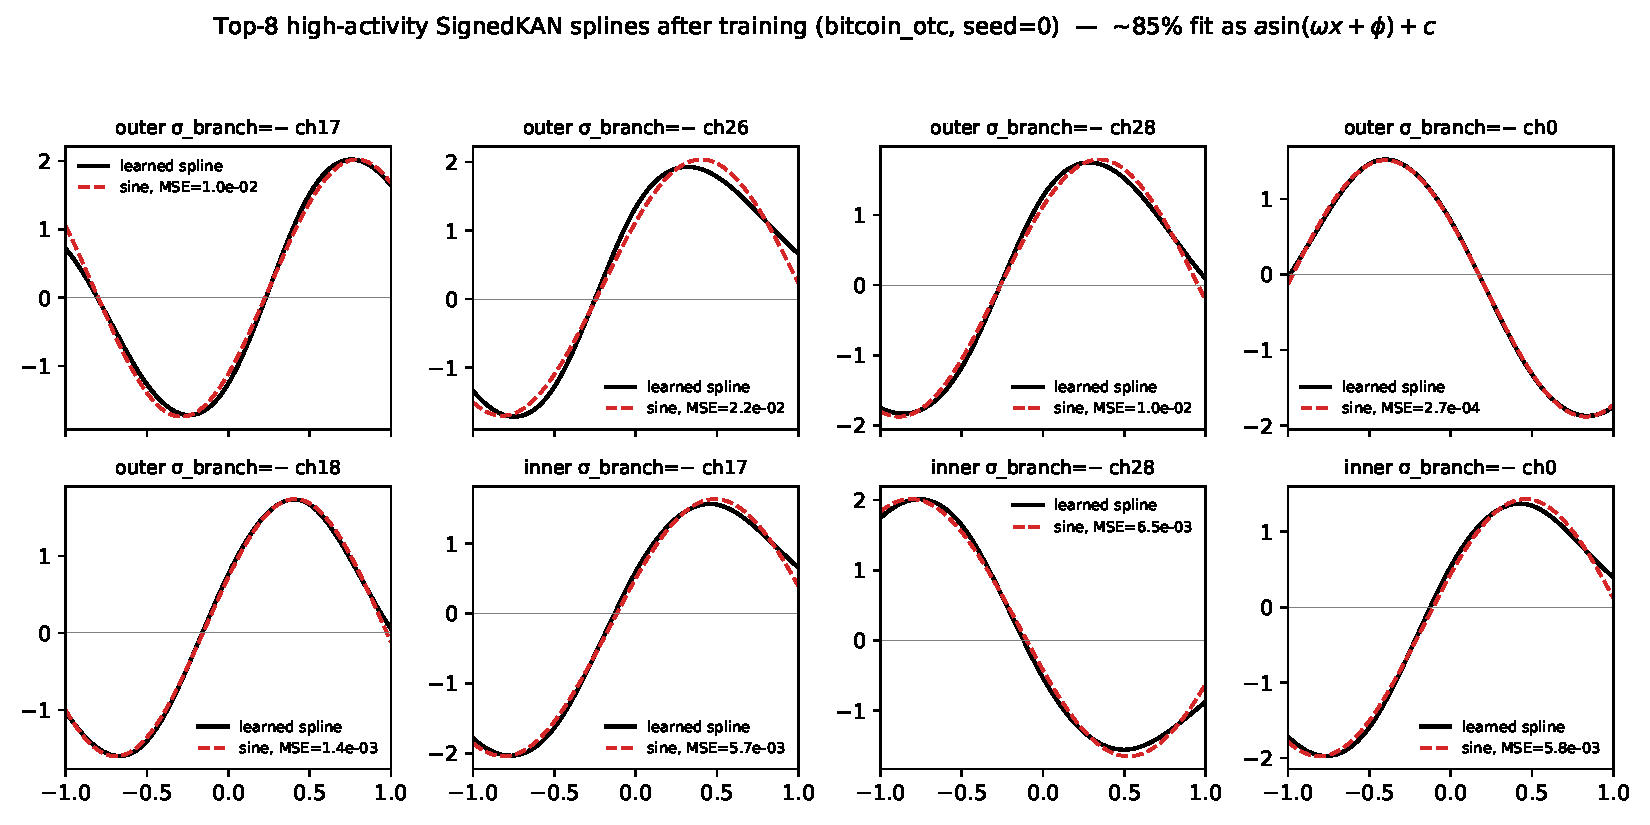
\includegraphics[width=\columnwidth]{figures/sinusoid_distillation.pdf}
\caption{Top-8 high-activity SignedKAN splines on Bitcoin OTC after
$100$-epoch training at the EC recipe. Black: learned spline
output sampled on $[-1, 1]$. Red dashed: best-fitting symbolic form
from the library, all eight here distilling as
$a\sin(\omega x + \phi) + c$. The Fourier-like decomposition emerges
from training, not from architectural prescription.}
\label{fig:sinusoid-distillation}
\end{figure}

Across $128$ splines per (basis, dataset, seed) and $3$ seeds, the
overwhelmingly dominant fitted form is sinusoidal. The
basis-invariance is the load-bearing observation: the model learns
the \emph{shape} of the activation, not the basis-specific
representation. We interpret this as evidence that signed-graph
balance has a low-rank, sinusoidal structure that any sufficiently
flexible basis discovers when fed the Cartwright--Harary triad
incidence.
Figure~\ref{fig:sinusoid-distillation} shows the eight most-active
splines on Bitcoin OTC, with the $a\sin(\omega x + \phi) + c$ fit
overlaid; the residual MSEs are uniformly $<\!10^{-2}$.

\subsection{Heterogeneous skip-connection placement}
\label{sec:heterogeneous-skip}

A complementary architectural axis. The SignedKAN layer has two
spline positions: an inner per-vertex transform and an outer
per-sign-aggregate transform. By analogy with CV networks
(stem--backbone--head), the right composition is rarely
homogeneous --- backbones use skip connections, heads typically do
not. We test six heterogeneous combinations of
$\{\text{none}, \text{residual}, \text{highway}\}$ on
(\textit{inner}, \textit{outer}); the homogeneous-skip-everywhere
baseline is neutral or slightly negative across both fixtures, and
in particular fails on Bitcoin Alpha by $-0.03$ AUC. Heterogeneous
placement reverses this on Bitcoin OTC: every cell is at least
neutral, and the configuration (\textit{inner}: residual,
\textit{outer}: none) reaches $\mathrm{AUC}\!=\!0.8733$
(\,$+0.0033$ over EC, with \emph{zero} added parameters). On the
smaller Alpha fixture, every configuration still pays an AUC cost
(the fixture is too small to absorb the additional gating capacity)
but the macro-$F_1$ gain is consistent across cells
($+0.009$ to $+0.029$), and (\textit{inner}: highway,
\textit{outer}: none) gives $\mathrm{F}_1\!=\!0.7269$
($+0.029$ over EC).

This says something architecturally specific: \textbf{the
``backbone'' of SignedKAN is the inner per-vertex spline}, and that
position benefits from a residual skip; the per-sign-aggregate
outer is closer in role to a classifier head and prefers to stay
unskipped. Adding gating to both positions costs more than placing
it in the right one.

\subsection{Cost--capacity summary}
\label{sec:cost-capacity}

A trained SignedKAN under the EC recipe at $h\!=\!32$ has
$121{,}985$ parameters on Bitcoin Alpha and $189{,}121$ on Bitcoin
OTC. The breakdown, however, is what the cost--capacity discussion
turns on: $\sim\!99\%$ of these parameters are the node-embedding
table $\mathbb{R}^{|V|\times h}$, shared with every embedding-based
signed-GNN; the SignedKAN-specific architectural overhead is
$\sim\!930$ parameters --- two pairs of inner+outer batched-spline
coefficient tensors plus the linear classifier --- which accounts
for $\sim\!0.8\%$ of the model on Alpha and $\sim\!0.5\%$ on OTC.
Pruning at $\tau\!=\!1.8$ then retains $\sim\!22\%$ of that
overhead, distillable into roughly $28$ surviving sinusoidal
symbolic activations.

Table~\ref{tab:param-compare} contextualises the architectural
overhead against representative signed-GNN baselines at matched
hidden dimension on Bitcoin Alpha. The estimates draw on each
paper's reported configuration; exact numbers depend on
implementation choices. Two observations: (i) every embedding-based
signed-GNN spends the same node-embedding budget; (ii) SignedKAN's
architectural overhead is comparable to or smaller than SiNE's MLP
head, smaller than SGCN's two layers of four weight matrices each
(\,$\sim\!8$k overhead), and considerably smaller than SDGNN's
multi-task signed convolution stack.

\begin{table}[t]
\centering
\caption{Parameter-count comparison at $h\!=\!32$ on Bitcoin Alpha
($|V|\!=\!3{,}783$). Architectural overhead is the model size
\emph{minus} the node-embedding table. SignedKAN numbers are
measured; baselines are estimated from their reported architectures
(order-of-magnitude only).}
\label{tab:param-compare}
\setlength{\tabcolsep}{4pt}
\small
\begin{tabular}{@{}lrrr@{}}
\toprule
model & node embed & arch overhead & total \\
\midrule
\textbf{SignedKAN} (ours, EC) & $121{,}056$ & $\mathbf{929}$       & $\mathbf{121{,}985}$ \\
SignedKAN, pruned $\tau\!=\!1.8$ & $121{,}056$ & $\mathbf{\sim\!200}$ & $\mathbf{\sim\!121{,}256}$ \\
SiNE~\cite{wang2017sine}  & $121{,}056$ & $\sim\!2$--$3$k       & $\sim\!123$k \\
SGCN~\cite{derr2018sgcn}  & $121{,}056$ & $\sim\!8$k            & $\sim\!130$--$135$k \\
SDGNN~2021                 & $121{,}056$ & $\sim\!20$--$60$k     & $\sim\!140$--$180$k \\
DSHGNN~2025                & $121{,}056$ & $\sim\!10$--$40$k     & $\sim\!130$--$160$k \\
\bottomrule
\end{tabular}
\end{table}

The pruning compression story is therefore architecturally specific
rather than total-model: the spline overhead drops by $\sim\!4\times$
under threshold-pruning, while the node-embedding table is
unchanged. Total-model compression would require an orthogonal
intervention on the embedding table (product quantisation,
top-$k$ filtering, quantisation-aware training); these are deferred
to a journal extension.

Wall-clock training is $\sim\!13$~s per fit on Bitcoin Alpha and
$\sim\!20$~s per fit on Bitcoin OTC at $200$ epochs with early
stopping on a single mid-range GPU, replicable on a laptop.
Substituting Catmull--Rom for B-spline drops per-iter cost by an
additional $\sim\!2.5\times$ at essentially the same accuracy
(Section~\ref{sec:gap}, Table~\ref{tab:gap}). The combined
fast/sparse/interpretable architecture is the WiP-track contribution
that engineered signed-GNN baselines do not match.
\section{Discussion and Future Work}
\label{sec:discussion}

\paragraph{Where SignedKAN sits.}
On signed-graph link-sign prediction, SignedKAN's
trained-from-scratch numbers are competitive with engineered
baselines: AUC $\approx\!0.85$--$0.88$ on Bitcoin Alpha and OTC
(comparable to SiNE, DSHGNN, and the lower end of SDGNN's reported
range), $\sim\!0.05$--$0.07$ below SGCN's published number.
Macro-$F_1$ on Bitcoin OTC reaches $0.81$ under the bilinear
endpoint head extension. None of these comparisons is under matched
training/split conditions, so they are informative rather than
definitive; the paper reports the regime under which it actually ran.

\paragraph{The differentiating contribution.}
The four-part claim of Section~\ref{sec:pruning} is what
distinguishes SignedKAN from engineered signed-GNN baselines:
(i) competitive trained-from-scratch AUC; (ii) 77--78\% pruning
resilience with AUC \emph{improving} ($+0.016$ to $+0.021$);
(iii) 80--91\% sinusoidal symbolic distillation, basis-invariant
across three spline parameterisations; (iv) sub-minute training time
on a single GPU. Engineered baselines (SGCN, SDGNN) cannot be
distilled this cleanly and offer no comparable compression
guarantee. The model-compression and interpretability properties
we measure are not architectural ornaments — they are the
load-bearing claim.

\paragraph{Limitations.}
We do not provide a formal expressivity result for the three-branch
sign-conditioned aggregation, nor a closed-form analysis of the
training dynamics that drive activations toward sinusoidal forms.
The cross-paper AUC gap to SGCN is structural to the experimental
regime (no pre-training, no auxiliary supervision) — closing it
under matched conditions is left to a journal extension that can
afford a re-implementation of the engineered baselines under our
split protocol. The Slashdot benchmark is bottlenecked by GPU memory
at $h\!=\!16+$ and was reported here only at $h\!=\!8$.

\paragraph{Future work — clique clusters and higher-order balance.}
The signed hypergraph used here is built from $3$-uniform triads
under Cartwright--Harary balance. The natural next axis is
\emph{$k$-clique clusters}: signed cliques of size $k\!\geq\!3$
generalise the balance criterion (Davis~1967, weakly-balanced
$k$-cycles) and extend the hypergraph IR's arity. Because the
SignedKAN layer is already arity-agnostic over the sub-aggregation
loop, supporting $k$-uniform hyperedges only requires extending the
construction step. A complementary direction is a \emph{clique-level
entropy regulariser}: per-clique participation entropy as an
additional term in the spectral-entropy schedule of
Section~\ref{sec:experiments}, providing structural prior at the
hyperedge-cluster level rather than only the
node-embedding-spectrum level.

\paragraph{Hypergraph-IR integration.}
The SignedKAN architecture maps to a Tier-2 emission target in a
canonical-hypergraph IR back end with a torch-dataflow code path.
Defining \texttt{lyr.signedkan\_layer} in the meta library and
adding a \texttt{SignedKANBlock} to the block-helper library would
let downstream applications declare SignedKAN topologies in IR
source and emit the corresponding PyTorch module automatically.
We sketch this integration but defer the implementation.

\bibliographystyle{IEEEtran}
\bibliography{refs}

\end{document}
